\documentclass[12pt]{article}
\usepackage[utf8]{inputenc}
\usepackage[margin=2cm]{geometry}
\usepackage{amsmath}
\usepackage{amssymb}
\usepackage{amsthm} % allows example and proof environment to be defined/used
\usepackage{cancel}
\usepackage{graphicx}
\usepackage{mathtools}
\usepackage[normalem]{ulem}
\newtheorem*{esempio}{Esempio}
\DeclarePairedDelimiter{\abs}{\lvert}{\rvert}

\begin{document}

\section[Lezione 10 - Ordine di convergenza]{Lezione 10 - Metodo di Newton parte 2, convergenza locale, ordine di convergenza, test di arresto, esempi, altri metodi di linearizzazione}
Partiamo dalla relazione chiave ottenuta nella lezione precedente per l'errore del metodo di Newton:
\[ e_{n+1} = c_n \cdot e_n^2 \leq c e_n^2 \]
\[ c_n = \frac{1}{2} \cdot \frac{\abs{\,f''(z_n)\,}}{\abs{\,f'(x_n)\,}}, \, c = \frac{1}{2} \cdot \frac{M_2}{m_1} \]
con $M_2 = \max\abs{\,f''(x)\,}$ e $m_1 = \min\abs{\,f'(x)\,}>0$ dove $x\in[c,d]$ assumendo che il metodo sia convergente, $f\in C^2[a,b]$ e che $\{ x_n\} \subset{[c,d]} \subseteq{[a,b]}$ con $f'(x)\neq0$ $\forall x\in[c,d]$ \\ 
Da questa abbiamo ottenuto, fissato $\theta\in (0,1)$ e preso $\bar{n}$ tale che 
\[ce_n\leq\theta<1 \quad \forall n\geq\bar{n} \quad \Longrightarrow \quad e_{\bar{n}+k}\leq\frac{1}{c}\,\theta^2, \quad k\geq0\] 
che ci ha fatto capire che per zeri semplici il metodo converge \uline{più che esponenzialmente}.

A questo punto possiamo chiederci: cosa succede se già con la scelta iniziale $x_0$ vale $ce_0<1$? In questo caso avremmo la disuguaglianza \[ ce_n\leq(ce_0)^{2^n} \]
con $n\geq0$. Infatti
\[\begin{split}
    ce_1 & \le (ce_0)^2 \\
    ce_2 & \le (ce_1)^2 \le (ce_0)^4 \\
    \vdots & \\
    ce_n & \le (ce_{n-1})^2 \le (ce_0)^{2^n}
\end{split}\]
Questo ci fa intuire che se $ce_0<1$ cioè 
\[e_0=\abs{\,x_0-\xi\,}<\frac{1}{c}\] 
cioè se prendiamo $x_0$ in un intorno opportuno di $\xi$ zero di $f$ avremo la convergenza con le sole ipotesi che $f \in C^2$ e che $f'(x) \neq 0$ in quell'intorno, perché 
\[ ce_0<1 \quad \Rightarrow \quad (ce_0)^{2^n} \to 0, n\to \infty \quad \Rightarrow \quad e_n \to 0, n \to \infty \]
Si può infatti dimostrare (non lo faremo per brevità) il seguente:

\subsection{TEOREMA (convergenza \uline{locale} del metodo di Newton)}
\begin{center}
    \fbox{\begin{minipage}[t]{15cm}%
        Sia $\xi$ zero di $f$ ed $ \exists\, \delta >0: f\in C^2(I_\delta)$ e $f'(x) \neq 0 \quad\forall x \in I_\delta$, dove $ I_\delta =[\xi-\delta,\xi+\delta]$; inoltre sia $ x_0 \in  (\xi - \gamma , \xi + \gamma) $ con  $\gamma=\min \left\{ \delta, \frac{1}{c}
        \right\} $ dove 
        \[c=\frac{1}{2}\cdot \frac{\max \abs{\,f''(x)\,}}{\min \abs{\,f'(x)\,}},\quad x\in I_\delta \]
        allora 
        \[ \forall n \geq 0 \quad x_n \in I_\gamma \quad \text{e} \quad e_n \leq \frac{1}{c} (ce_0)^{2^n} \underset{n\to \infty}{\longrightarrow} 0\]
    \end{minipage}}
\end{center}
(nella dimostrazione, per chi volesse provare a farla, un punto chiave è far vedere per induzione che se $x_n \in I_\gamma \Rightarrow x_{n+1}\in I_\gamma$, a cui si arriva mostrando che  $e_{n+1}<e_n<\gamma \ \forall n$ ).
\newline \newline
Come abbiamo già osservato nella lezione precedente, il metodo di Newton pur essendo molto veloce sarebbe poco utile se funzionasse solo in ipotesi forti come ad esempio quelle del teorema di convergenza globale, in cui $e_0$ può può essere grande ma le ipotesi su $f$ sono molto restrittive ($f''$ di segno costante in $[a,b]$).\\
Invece nel teorema di convergenza locale  (che di nuovo, vale la pena di ribadirlo, è un set di condizioni sufficienti (non necessarie) per la convergenza) basta che $ f\in C^2$  e  $ f'\neq 0 $ in un intorno di  $ \xi $ , con la seconda ipotesi che é sempre soddisfatta se lo \uline{zero} è \uline{semplice} perché $f'$ è continua (permanenza del segno di $f'(\xi)$).\\
Conviene a questo punto formalizzare il concetto di ``convergenza quadratica" del metodo di Newton, dando delle definizioni generali sull'ordine di convergenza di un metodo. 

\subsection{DEFINIZIONE \uline{(ordine di convergenza)}}
\begin{center}
    \fbox{\begin{minipage}[t]{17cm}%
Dato un metodo che produce una successione $\{x_n\}_{n\geq 0} $  tale che $\lim_{n \to \infty}x_n=l $  con $l$ limite finito si dice che: 
\begin{enumerate}
\item  il metodo ha ordine di convergenza \uline{almeno} $p \geq 1$ se $ \exists\, c>0$ con ($ c \in (0,1) $ se $p=1$) tale che 
\[e_{n+1}\leq ce_n^p \quad \forall n\]
\item  il metodo ha ordine di convergenza \uline{esattamente} $p\geq 1$ se  $\exists  L>0$ (con $ L\in (0,1)$ se $p=1$ ) tale che:
\[ \lim_{n\to\infty}\frac{e_{n+1}}{e_n^p}=L\]
(dove $L$ è spesso chiamata \uline{costante asintotica} del metodo).\\ 
La convergenza è detta \uline{lineare} se $p=1$, \uline{superlineare} se $p>1$ e in particolare \uline{quadratica} se $p=2$,  \uline{cubica} se $p=3$, $\dotso$
\end{enumerate}
\end{minipage}}
\end{center}
Facciamo alcune osservazioni: nel caso $p=1$ le condizioni $e_{n+1} \leq ce_n, 0<c<1$  (convergenza almeno lineare) e $\lim_{n\to\infty}{\frac{e_{n+1}}{e_n}}=L$ con $L\in(0,1)$ sono condizioni sufficienti per la convergenza. Infatti da $e_{n+1}\leq ce_n$ si ricava 
\[\begin{split}
    e_1 & \leq ce_0, \\
    e_2 & \leq ce_1 \leq c^2e_0, \\
    e_3 & \leq ce_2 \leq c^3e_0, \\
    & \dotso \\
    e_n & \leq c^ne_0
\end{split}\] 
con $c^n\rightarrow 0,n\rightarrow\infty$ perché $c\in[0,1]$ da cui $e_n\rightarrow 0, n\rightarrow\infty$. \\
Analogamente, se $\lim_{n\to \infty}{\frac{e_{n+1}}{e_n}}=L$ con $L\in(0,1)$, preso $\overline{\varepsilon}\in(0,1-L)$ $\exists\, \overline{n}$ tale che 
\[0\leq\frac{e_{n+1}}{e_n}\leq L+\overline{\varepsilon}=c<1 \quad\forall n \geq \overline{n}\] 
cioè $e_{n+1}\leq ce_n$ $\forall n\geq\overline{n}$, da cui ragionando come sopra $e_n \leq c^{n-\overline{n}}e_{\overline{n}} \rightarrow 0$, $n\rightarrow\infty$.\\
D'altra parte, se c'è convergenza, allora necessariamente $L\le 1$.\\
Infatti, se $\lim_{n \to \infty} \frac{e_{n+1}}{e_n} = L > 1$, preso $\overline{\varepsilon} \in (0, L-1)$ $ \exists\, \overline{n}$ tale che $1<L-\overline{\varepsilon} \leq \frac{e_{n+1}}{e_n}$ $\forall n \geq \overline{n}$, quindi $e_{n+1} \geq (L-\overline{\varepsilon})\cdot e_n$ da cui 
\[e_{\overline{n}+1} \geq (L-\overline{\varepsilon}) \cdot e_{\overline{n}}, \dotso, e_n \geq (L-\overline{\varepsilon})^{n-\overline{n}} e_{\overline{n}} \to \infty, n \to \infty\]
e l'errore divergerebbe, cioè non ci sarebbe convergenza.

\subsection{Ordine di convergenza metodo di Newton}
Per quanto riguarda il metodo di Newton, dalla definizione di ordine di convergenza possiamo dire che l'ordine è almeno $p=2$ per zeri semplici perché sappiamo che in tal caso $e_{n+1} \leq ce^2_n$; d'altra parte dall'analisi fatta sappiamo che
\[\frac{e_{n+1}}{e_n^2} = c_n = \frac{1}{2} \cdot \frac{\abs{\,f''(z_n)\,}}{\abs{\,f'(x_n)\,}} \to \frac{1}{2} \cdot \frac{\abs{\,f''(\xi)\,}}{\abs{\,f'(\xi)\,}}\]
per $n \to \infty$ (visto che $z_n \in int(\xi,x_n)$ e $f', f''$ sono continue quindi lo sono $\abs{\,f'\,}, \abs{\,f''\,}$ e si può portare il limite ``dentro le funzioni").\\
Ma allora l'ordine è esattamente $p=2$ se $f''(\xi) \neq 0$, altrimenti $L=0$ e si può dimostrare (non lo faremo) che l'ordine è almeno $p=3$ se $f$ ammette derivata terza in $\xi$.
\newline \newline
Vale la pena di notare che il metodo di bisezione, pur comportandosi ``in media" come un metodo di ordine $p=1$ e costante asintotica $L=1/2$, non ha un ordine definito.\\
Infatti in generale non si può dimostrare che $\exists c: e_{n+1} \leq c\cdot e_n$ con $0<c<1$ e tanto meno che $\lim_{n\to \infty} \frac{e_{n+1}}{e_n} = \frac{1}{2}$.\\
Facciamo infine un'ultima osservazione sull'ordine di convergenza del metodo di Newton: cosa succede quando  $f'(\xi) = 0$ cioè quando lo zero non è semplice?\\
In questo caso l'ordine di convergenza del metodo di Newton scende a $p=1$ con costante asintotica $1-\frac{1}{m}$ dove $m$ è la molteplicità dello zero, cioè $f(\xi) = f'(\xi) = \cdots = f^{(m-1)}(\xi) = 0$ e $f^{(m)}(\xi) \neq 0$.\\
Ad esempio, se $m=2$, cioè se $f'(\xi) = 0$ e $f''(\xi) \neq 0$ si ha
\[\frac{e_{n+1}}{e_n} = \frac{e_{n+1}}{e_n^2} \cdot e_n = c_n \cdot e_n = \frac{1}{2} \cdot \frac{\abs{\,f''(z_n)\,}}{\abs{\,f'(x_n)\,}} \cdot e_n\]
Usando la formula di Taylor
\[ f'(x_n)=\underbrace{f'(\xi)}_{=0} + f''(\xi)\cdot (x_n - \xi)+o(e_n) \]
(dove $\alpha_n = o(\beta_n)$ significa che $\lim_{n \to \infty} \frac{\alpha_n}{\beta_n} = 0$), da cui
\[\frac{\abs{\,f'(x_n)\,}}{e_n} \to \abs{\,f''(\xi)\,}, \quad n \to \infty\]
e quindi
\[ \frac{e_{n+1}}{e_n} = e_n \cdot c_n \to \frac{1}{2}, \quad n \to \infty \]

\subsubsection{Perché nel calcolo di $\sqrt2$ con Newton il numero di cifre corrette raddoppia ad ogni iterazione?}
Dopo questo ``excursus" sulla importante nozione di ordine di convergenza, applicata al metodo di Newton, vediamo di spiegare come mai nel caso del calcolo di $\sqrt{2}$ il numero di cifre corrette essenzialmente raddoppia ad ogni iterazione.\\
Quando si parla di cifre corrette, che sono cifre di mantissa, si sta parlando sostanzialmente dell'errore relativo 
\[r_n = \frac{e_n}{\abs{\,\xi\,}}, \quad \xi \neq 0\]
Ora, da $e_{n+1} \leq ce_n^2$ otteniamo 
\[ r_{n+1} = \frac{e_{n+1}}{\abs{\,\xi\,}} \leq c\,\frac{e_n^2}{\abs{\,\xi\,}} = c\,\abs{\,\xi\,}\,r_n^2 \]
Se $c\abs{\,\xi\,} \leq 1$ si ha $r_{n+1} \leq r^2_n$, cioè l'errore \uline{relativo} al passo $n+1$ è maggiorato dal quadrato dell'errore relativo al passo $n$
\[\begin{split}
    r_1 & \leq r_0^2,\\
    r_2 & \leq r_1^2 \leq r_0^4,\\ 
    & \vdots \\ 
    r_n & \leq r_{n-1}^2 \leq r_0^{2^n}
\end{split}\]
Per fissare le idee, se al passo $k$ $r_k < 10^{-1}$, avremo $r_{k+1} < 10^{-2}$, $r_{k+2} < 10^{-4}$, $r_{k+3} < 10^{-8}$ e con $r_{k+4} < 10^{-16}$ siamo già sotto la precisione macchina. \\
Questo è proprio quanto succede con $f(x) = x^2 - 2$ in $[\sqrt{2},2]$, dove 
\[ c = \frac{1}{2}\frac{2}{\underset{x \in [\sqrt{2},2]}{\min}2x}  = \frac{1}{2} \cdot \frac{2}{2\sqrt{2}} = \frac{1}{2\sqrt{2}} \]
\[c\,\abs{\,\xi\,} = \frac{\sqrt{2}}{2\sqrt{2}} = \frac{1}{2} < 1\]
e
\[ r_1 = \frac{1.5 - \sqrt{2}}{\sqrt{2}} \approx 0.06 < 10^{-1} \]
infatti $r_5 < 10^{-16} \Rightarrow x_5 = fl(\sqrt{2})$.

\subsection{Step e residuo pesato}
Prima di fare un paio di esempi ulteriori, è bene discutere alcuni aspetti implementativi.\\
Innanzitutto, osserviamo che richieste computazionali del metodo di Newton sono molto più forti di quelle del metodo di bisezione.\\
Se la bisezione infatti nella versione base ha bisogno solo di conoscere il segno di $f(x)$ (per cui basta come sappiamo errore $< 100\%$ sulla quantità) e col test del residuo pesato (che assume zero semplice e $f \in C^1$) basta saper stimare l'ordine di grandezza del residuo e del peso, ovvero l'ordine di grandezza di $f$ ed $f'$ almeno per $n$ abbastanza grande (infatti per la derivata possiamo accontentarci di una stima tramite rapporti incrementali), col metodo di Newton diventa essenziale poter calcolare con accuratezza sia $f(x_n)$ che $f'(x_n)$ perché gli errori su queste quantità tendono ad essere dominanti nel processo iterativo di calcolo. \\
D'altra parte per il metodo di Newton non abbiamo una stima a priori facile da usare per arrestare le iterazioni.\\
Pensiamo infatti, ad esempio, al caso della convergenza locale e alla stima $e_n \leq \frac{1}{c} \cdot (c\cdot e_0)^{2^n}$.\\
Questa ci dice qualitativamente che c'è convergenza prendendo $x_0$ in un intorno di $\xi$, ma per trovare tale intorno e per usare la stima avremmo bisogno di conoscere $c$, che richiede di saper stimare il minimo di $\abs{f'}$ ma anche il max di $\abs{f''}$ (il che è agevole quando di $f$ sia nota un'espressione analitica semplice ma non in generale).\\
Per fortuna il metodo di Newton può sfruttare una semplice stima a posteriori, il cosiddetto ``STEP" $\abs{x_{n+1} - x_n}$ (la distanza tra le ultime 2 iterazioni).\\
Quando si ha a che fare con un metodo convergente, lo step va a zero per $n \to \infty$ perché $x_n, x_{n+1} \to \xi$; ma una stima dell'errore basata sullo step non è affidabile in generale (anche se stavolta viene usata come stima empirica tipo ``ultima spiaggia").\\
Invece col metodo di Newton lo step è una stima molto buona per costruzione, almeno per $n$ abbastanza grande, perché
\[ STEP(n) = \abs{x_{n+1} - x_n} = \frac{\abs{f(x_n)}}{\abs{f'(x_n)}} \]
visto che 
\[x_{n+1} = x_n - \frac{f(x_n)}{f'(x_n)}\]
cioè per Newton lo \uline{STEP} è per costruzione un \uline{RESIDUO PESATO} ed è già in pratica calcolato ad ogni iterazione visto che basta prendere il modulo di $\frac{f(x_n)}{f'(x_n)}$ che è una quantità chiave nel processo di calcolo.\\
In effetti, la stima a posteriori dello step è generalmente affidabile, soprattutto quando è accompagnata da altri controlli di convergenza.\\
Infatti, sia nel teorema di convergenza globale che in quello di convergenza locale si vede che l'\uline{errore} è \uline{decrescente} ($e_{n+1} < e_n$): quindi per avere garanzia di essere in condizioni di convergenza si può controllare per prima cosa che lo step sia decrescente e poi usarlo come stima accurata dell'errore non appena $\abs{f'(x_n)}$ comincia a stabilizzarsi cioè 
\[\frac{\abs{f'(x_{n-1})}}{\abs{f'(x_n)}} \approx 1\] 
(criterio empirico che abbiamo già discusso nella stima del residuo pesato per il metodo di bisezione).\\
Questo approccio può essere particolarmente utile se si usa un metodo cosiddetto ``ibrido", come sono di solito i metodi adottati dai solutori automatici di equazioni, che in input richiedono $f$, $x_0$ e una tolleranza, accoppiando un metodo ``lento" ma affidabile (ad es. bisezione) per fare alcune iterazioni, partendo poi con un metodo veloce (ad es. Newton o sue varianti) con un controllo di convergenza (tipo decrescita dello step per Newton) e iterando il procedimento finché il metodo veloce non entra in condizioni di convergenza rapida perché parte dell'intorno ``giusto" dello zero (intorno non noto a priori), arrestando le iterazioni con una stima a posteriori (lo step per Newton).\\
Sempre parlando di approccio empirico all'implementazione di un metodo iterativo convergente (non necessariamente un metodo per la soluzione di equazioni) siamo interessati in pratica all'errore relativo, a meno che $\xi = 0$ (o sia piccolissimo).\\
Per avere un test di arresto che funzioni sia per $\xi \neq 0$ (dove conta l'errore relativo) sia per $\xi \approx 0$ (dove conta l'errore assoluto), avendo una stima affidabile dell'errore assoluto si usa spesso un test del tipo
\[stima(n) \leq \varepsilon_a + \abs{x_n} \cdot \varepsilon_r\]
dove $\varepsilon_a$ è una tolleranza assoluta e $\varepsilon_r$ una tolleranza relativa (ad es. $\varepsilon_a = 10^{-10}$, $\varepsilon_r = 10^{-8}$).\\
In questo modo, visto che $\abs{x_n} \to \abs{\xi}$, se $\xi$ è  ben staccato da zero ci si ferma su $\varepsilon_r$, se $\xi = 0$ (oppure $\xi$ è ``piccolissimo") ci si ferma su $\varepsilon_a$.\\
Vediamo come si comporta la stima dello step per il metodo di Newton nel calcolo di $\sqrt{2}$
\begin{center}
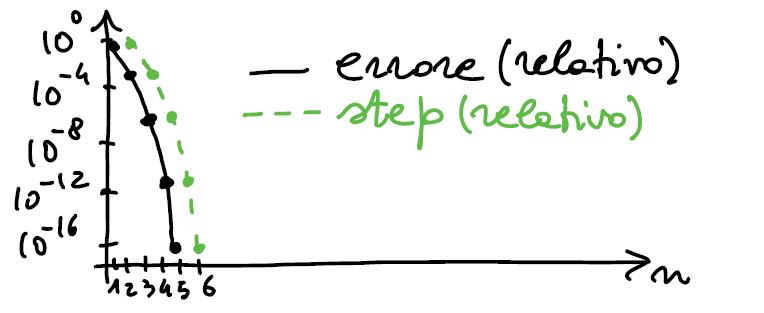
\includegraphics[width=0.5\textwidth]{pag27.JPG}
\end{center}
Si vede che la curva dello step è ``parallela" alla curva dell'errore (quindi è un'ottima stima) ma risulta slittata in avanti di 1: questo è naturale, visto che per avere il residuo pesato $\frac{\abs{f(x_n)}}{\abs{f'(x_n)}}$ al posto di $n$ bisogna essere arrivati al passo $n+1$, 
\[x_{n+1} - x_n = - \frac{f(x_n)}{f'(x_n)}\]
Siccome l'errore decresce velocemente, la stima dello step diventa ancora più affidabile
\[ r_{n+1} = \frac{e_{n+1}}{\abs{\xi}} \ll r_n = \frac{e_n}{\abs{\xi}} \approx \frac{\abs{x_{n+1} - x_n}}{\abs{\xi}}\]
Facciamo ora due esempi di applicabilità del metodo di Newton.

\subsection{Esempio 1 - Metodo di Erone per le radici quadrate}
Abbiamo visto come usare il metodo di Newton per calcolare $\sqrt{2}$ come soluzione dell'equazione algebrica (zero di un polinomio) $f(x) = x^2 - 2 = 0$.\\
L'approccio è generalizzabile al calcolo di $\sqrt{a}$, $a>0$, risolvendo l'equazione $x^2 - a = 0$.\\
Osserviamo che $f(0) = - a < 0$ e $f(b) > 0$ per $b^2 > a$.\\
Visto che $f'(x) = 2x$ e inoltre $f''(x) = 2 > 0$ siamo nelle ipotesi del teorema di convergenza globale scegliendo $x_0$: $x^2_0 > a$.\\
Qual è la forma delle iterazioni di Newton in questo caso?
\[\begin{split}
    x_{n+1} & = x_n - \frac{f(x_n)}{f'(x_n)} \\
    & = x_n - \frac{x_n^2-a}{2 x_n} \\
    & = \frac{2 x_n^2 - x_n^2 + a}{2 x_n} \\
    & = \frac{x_n^2 + a}{2 x_n} \\
    & = \frac{x_n}{2} + \frac{a}{2 x_n}, \quad n \ge 0
\end{split}\]
Quindi se $a$ è razionale (in particolare intero) e $x_0$ è razionale il metodo fornisce per costruzione una successione di razionali (frazioni) che converge a $\sqrt{a}$ (quadraticamente perché $\sqrt{a}$ è zero semplice).\\
Questa iterazione era già nota in età ellenistica ed è attribuita al matematico greco Erone di Alessandria (che vi era arrivato non col calcolo differenziale, ignoto all'epoca, ma con metodi geometrici).\\
Lasciamo come ulteriore esercizio la generalizzazione al calcolo di $\sqrt[k]{a} = a^{\frac{1}{k}}$, $k>0$ (ad esempio radice cubica, $k=3$) e anche implementazione e test in Matlab.

\subsection{Esempio 2 - Applicazione del metodo di Newton a un'equazione trascendente}
Il metodo di Newton è applicabile (nelle giuste ipotesi) a qualsiasi equazione del tipo $f(x)=0$ , quindi anche ad equazioni in cui $f$ non è un polinomio o una funzione razionale (rapporto di polinomi), dette equazioni trascendenti (quelle polinomiali/razionali sono dette equazioni algebriche).\\
È il caso di osservare che in realtà anche le equazioni algebriche richiedono metodi numerici: infatti è noto (teoria di Galois) che gli zeri di polinomi di grado $\geq 5$ non sono calcolabili tramite radicali e d'altra parte le stesse equazioni di $2^{\circ}$ grado richiedono il calcolo di $\sqrt{\Delta}$ che va fatto con un metodo approssimato (abbiamo visto sopra come usare Newton che è molto veloce per le radici quadrate). \\
Consideriamo l'equazione trascendente: 
\[f(x)=x-e^{-\alpha x}=0 ,\quad \alpha>0 \]
che si può interpretare come intersezione di grafici (in effetti ha banalmente la forma di punto fisso $x=e^{-\alpha x}$ e la useremo anche nella prossima lezione).\\
Osserviamo che $f \in C^{\infty}(\mathbb{R})$ , $f(0)=-1<0$ , $f(1)=1-e^{-\alpha}>0$ quindi $\exists \  \xi \in (0,1):\ f(\xi)=0$\\
Lo zero è sicuramente unico (in $\mathbb{R}$)\\
\[f'(x)=1+\alpha e^{-\alpha x}>0 \quad \text{($f$ è strettamente crescente)}\]
inoltre \[f''(x)=-\alpha^2 e^{-\alpha x}<0 \quad \text{($f$ è strettamente concava)}\]
\begin{center}
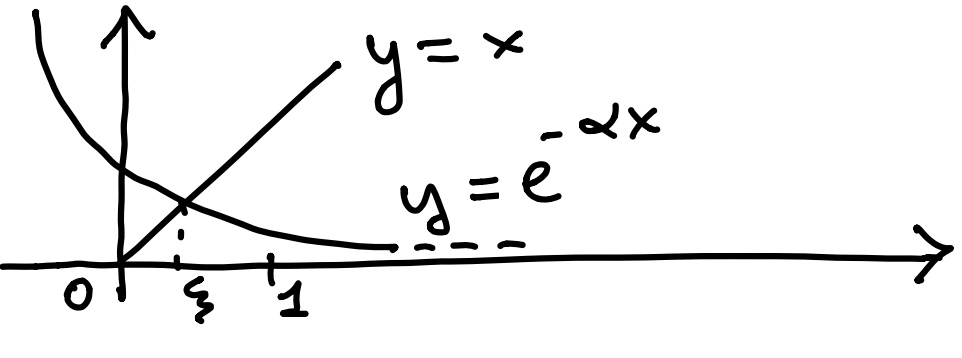
\includegraphics[width=0.5\textwidth]{pag34.png}
\end{center}
Inoltre 
\[ f'(x) \geq f'(1) = 1+ \alpha e^{-\alpha} \]
e
\[ \abs{f''(x)} = \alpha^2 e^{-\alpha x} \leq \alpha^2, \quad x\in[0,1] \]
vale quindi
\[ c = \frac{1}{2}\,\frac{M_2}{m_1} \leq \frac{1}{2}\,\frac{\alpha^2}{1+\alpha e^{-\alpha}} \]
per $\alpha \leq 1$ abbiamo che 
\[ c\,\abs{\xi} < \frac{1}{2} \]
da cui otteniamo
\begin{equation*}
    r_{n+1} = \frac{e_{n+1}}{\abs{\xi}} < \frac{1}{2}r_n^2
\end{equation*}
e anche in questo caso ci sarà un raddoppio (almeno) delle cifre corrette ad ogni iterazione (per $\alpha = 1$, $x_5=fl(\xi)=0.5671432904097838$).\\
Lasciamo come esercizio i test in Matlab su questa equazione.

\subsection{Metodo delle corde e delle secanti}
Concludiamo la lezione mostrando in breve altri 2 metodi classici per la soluzione numerica di equazioni non lineari, anch'essi basati su una forma di \uline{LINEARIZZAZIONE} iterativa, il metodo delle CORDE e il metodo delle SECANTI:
\begin{center}
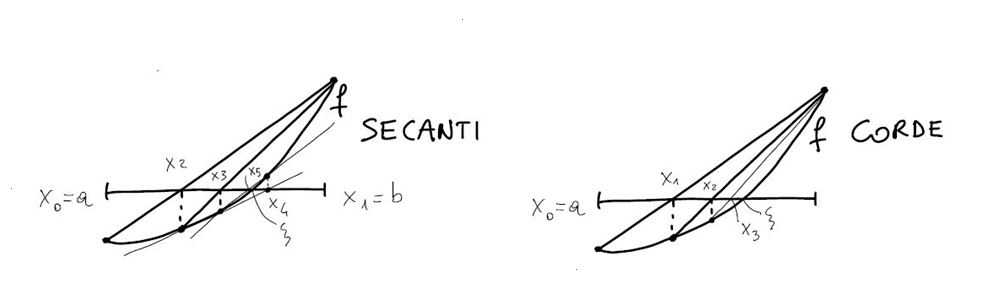
\includegraphics[width=\textwidth]{pag36.JPG}
\end{center}
Entrambi i metodi corrispondo a sostituire l'equazione $f(x)=0$ con un'equazione lineare
\[ f(x_n)+q_n(x-x_n)=0 \]
dove nel metodo delle corde $q_n$ è il coefficiente angolare della corda (segmento) per $(x_n,f(x_n))$ e $(b,f(b))$
\[ q_n=\frac{f(b)-f(x_n)}{b-x_n} \]
mentre nel metodo delle secanti $q_n$ è il coefficiente angolare della retta per $(x_{n-1},f(x_{n-1}))$ e $(x_n,f(x_n))$
\[ q_n=\frac{f(x_n)-f(x_{n-1})}{x_n-x_{n-1}} \]
(osserviamo che nel metodo di Newton $q_n=f'(x_n)$).\\
Entrambi i metodi hanno ipotesi di convergenza globale e locale, ad esempio il metodo delle corde converge se $f''$ ha segno costante e $x_0$ è tale che $f(x_0)f''(x_0)>0$; inoltre, il metodo delle corde ha convergenza lineare ($p=1$) mentre il metodo delle secanti ha convergenza superlineare con $p\in(1,2)$. \\
In effetti ci aspettiamo che il metodo delle secanti sia più veloce, perché entrambi rispetto a Newton hanno un rapporto incrementale al posto della derivata
\[ x_{n+1}=x_n-\frac{f(x_n)}{q_n} \]
con $n\geq0$ (corde) e $n\geq1$ (secanti), ma mentre nelle corde un estremo è fisso, nelle secanti per $f\in C^1$
\[ q_n=\frac{f(x_n)-f(x_{n-1})}{x_n-x_{n-1}}\overset{\overset{valor}{medio}}{=} f'(u_n) \]
con $u_n\in int(x_n,x_{n-1})$, quindi se c'è convergenza per il teorema dei 2 carabinieri $u_n\rightarrow\xi$, $n\rightarrow\infty$ e $q_n \rightarrow f'(\xi),\, n\rightarrow\infty$, cioè la secante tende ad essere sempre più ``simile" ad una tangente al crescere di $n$.\\In effetti si può dimostrare (non lo faremo, la dimostrazione richiede nozioni sull'interpolazione lineare che ancora non abbiamo) che l'ordine di convergenza del metodo delle secanti è
\[ p=\frac{1+\sqrt{5}}{2}=1.618\dotso\]
la famosa ``sezione aurea", un numero molto importante in matematica che si incontra in numerose questioni sia teoriche che applicative.\\
Non è difficile far vedere (facoltativo) che per $p>1$ da 
\[ e_{n+1}\leq ce_n^{p} \]
si ricava che $\exists\, c'>0$ tale che
\[ c'e_n\leq(c'e_0)^{p^n} \]
Quindi per $c'e_0<1$ la convergenza è molto rapida (meno di quella di Newton perchè $p<2$ ma comunque più che esponenziale).\\Il metodo delle secanti risulta quindi una valida alternativa al metodo di Newton quando $f'$ non sia nota o difficile da calcolare (e come Newton è generalizzabile a \uline{sistemi} di equazioni non lineari).
\end{document}

